% =============================================================================
% IJCRSEE-format report: SANF-Net for EEG-based dementia and MCI detection
% Layout follows the IJCRSEE Word template (IJCRSEEtemplate.doc):
%   A4, margins 2.5 cm, header/footer 1.5 cm, single spacing, justified,
%   Arial Narrow (here: Helvetica Narrow) 16 pt title, 10 pt abstract/keywords,
%   12 pt body, 10 pt hanging references, APA citations, max. three heading levels.
% Compile: tectonic main.tex   (or pdfLaTeX + BibTeX on Overleaf)
% Each section lives in sections/*.tex
% =============================================================================
\documentclass[12pt,a4paper]{article}

\usepackage[a4paper,left=2.5cm,right=2.5cm,top=2.5cm,bottom=2.5cm,
            headsep=0.6cm,footskip=1.5cm]{geometry}
\usepackage[T1]{fontenc}
\usepackage[scaled=1.0]{helvet}            % Helvetica stands in for Arial
\renewcommand{\familydefault}{\sfdefault}
\renewcommand{\mddefault}{mc}               % narrow (condensed) medium weight
\renewcommand{\bfdefault}{bc}               % narrow bold
\usepackage{sansmath}\sansmath
\usepackage{amsmath,amssymb}
\usepackage{graphicx}
\usepackage{booktabs,multirow,array,tabularx}
\usepackage{xcolor}
\usepackage{tikz}
\usetikzlibrary{positioning}
\usepackage[round,authoryear]{natbib}
\usepackage{url}
\usepackage[hidelinks]{hyperref}
\usepackage{caption}
\usepackage{titlesec}
\usepackage{fancyhdr}
\usepackage{enumitem}
\usepackage{float}

% --- placeholders (remove all before submission) ------------------------------
\newcommand{\todo}[1]{\textcolor{red}{[TODO: #1]}}

% --- paragraphs: justified, single spaced, no space between paragraphs -------
\setlength{\parskip}{0pt}
\setlength{\parindent}{1.25cm}
\linespread{1.0}

% --- headings: max three levels, bold, no numbering (IJCRSEE style) ----------
\setcounter{secnumdepth}{0}
\titleformat{\section}{\normalfont\fontsize{12}{14}\bfseries}{}{0pt}{}
\titleformat{\subsection}{\normalfont\fontsize{12}{14}\bfseries\itshape}{}{0pt}{}
\titleformat{\subsubsection}{\normalfont\fontsize{12}{14}\itshape}{}{0pt}{}
\titlespacing*{\section}{0pt}{12pt}{6pt}
\titlespacing*{\subsection}{0pt}{9pt}{4pt}
\titlespacing*{\subsubsection}{0pt}{6pt}{3pt}

% --- tables and figures: "Table 1" on its own line, caption below it ---------
\captionsetup[table]{labelsep=newline,justification=raggedright,singlelinecheck=false,
                     font={small},labelfont=bf,textfont=it}
\captionsetup[figure]{labelsep=period,font={small},labelfont=bf}

% --- references: 10 pt, hanging indent ----------------------------------------
\setlength{\bibsep}{2pt}
\renewcommand{\bibfont}{\fontsize{10}{12}\selectfont}
\setlength{\bibhang}{1.25cm}

% --- page style ------------------------------------------------------------------
\setlength{\headheight}{14pt}
\pagestyle{fancy}
\fancyhf{}
\renewcommand{\headrulewidth}{0pt}
\fancyfoot[C]{\small\thepage}
\fancyhead[R]{\footnotesize Potdar, S. et al. (2026). Dementia detection using state-aware, age-normative EEG classification}

\begin{document}

% ============================ title block =======================================
\thispagestyle{empty}
\noindent{\footnotesize
\begin{tabularx}{\textwidth}{@{}X r@{}}
\textbf{Original scientific paper} & \\
Received: November 3, 2026. & \\
\end{tabularx}}

\vspace{10pt}
\begin{center}
{\fontsize{16}{19}\selectfont\bfseries Dementia Detection Using State-Aware, Age-Normative EEG Classification
with a Lightweight Fusion Network\par}
\vspace{10pt}
{\fontsize{12}{14}\selectfont Siddarth Potdar$^{1*}$, Sanchit Raut$^{1}$, Vedant Kannurkar$^{1}$\par}
\vspace{4pt}
{\fontsize{10}{12}\selectfont $^{1}$Department of Computer Science and Engineering, Sardar Patel Institute of
Technology, Mumbai, India, \{siddarth.potdar23, sanchit.raut23, vedant.kannurkar24\}@spit.ac.in\par}
\end{center}

\vspace{6pt}
{\fontsize{10}{12}\selectfont\setlength{\parindent}{0pt}
% Abstract: max. 250 words, no abbreviations, no formulas (IJCRSEE rule).
\noindent\textbf{Abstract:} Resting-state electroencephalography is an inexpensive, portable candidate for
screening mild cognitive impairment and dementia, but published deep learning models are large, mix
different recording states and are rarely tested outside their own dataset. This study aimed to build a
compact, interpretable classifier of normal cognition, mild cognitive impairment and dementia and to evaluate
it rigorously. Using 1,187 clinical recordings from Chung-Ang University Hospital, we first corrected a timing
error in the event annotations, reducing the median misalignment in paused recordings from 33 to 3 seconds
and making the eyes-closed, eyes-open and light-stimulation state of every second known. We then designed a
state-aware, age-normative fusion network with 143,000 parameters that combines state-conditioned signal
segments, 48 clinical biomarkers expressed relative to healthy people of the same age, and age, through
interpretable gates. An ensemble of three networks reached 72.9\% accuracy and an area under the curve of 0.87
on the official test split, above the best published single model (70.2\%) at a fraction of its size, and
recognised 95.7\% of healthy participants. Under repeated five-fold cross-validation the network reached
59.5\%, matching logistic regression on the same biomarkers and exceeding two deep learning baselines.
Community volunteers were younger and recorded with a different stimulation protocol than patients, which
inflates apparent performance, and the model transferred to an independent cohort with an area under the curve
of 0.70. We recommend confound-controlled, cross-validated evaluation for such screening tools.

\vspace{6pt}
\noindent\textbf{Keywords:} electroencephalography, dementia, mild cognitive impairment, deep learning,
normative modelling, human--AI interaction.

\par}

% first-page footnote (corresponding author + licence), as in the template
\begingroup
\renewcommand{\thefootnote}{}
\footnotetext{\hspace{-1.8em}\footnotesize *Corresponding author: siddarth.potdar23@spit.ac.in\\[2pt]
\copyright\ 2026 by the authors. This article is an open access article distributed under the terms and
conditions of the Creative Commons Attribution (CC BY) license
(\url{https://creativecommons.org/licenses/by/4.0/}).}
\endgroup

% ============================== body ============================================
\section{Introduction}

Dementia affects about 57 million people worldwide, a number projected to rise to about 153 million by 2050
\citep{who2023dementia}; in India alone, cases are expected to grow from 5.1 million in 2021 to more than 20
million by 2050. Mild cognitive impairment (MCI) is the main prodromal stage of dementia \citep{petersen2004mci},
and it is the window in which intervention is most useful. Neuropsychological testing, magnetic resonance
imaging (MRI), positron emission tomography and cerebrospinal fluid biomarkers are costly, invasive or scarce
outside large hospitals. Scalp electroencephalography (EEG), in contrast, is cheap, portable, non-invasive and
widely available. Alzheimer's-type dementia produces well-documented EEG changes: slowing of the background
rhythm, reduced posterior alpha, increased theta and delta power, and reduced coherence
\citep{jeong2004eeg,dauwels2010diagnosis,babiloni2020measures}.

The CAUEEG dataset \citep{kim2023caueeg} is one of the largest public clinical EEG collections with a
Normal / MCI / Dementia benchmark. Results on it are, however, hard to interpret for four reasons. First,
clinical EEG slowing is read during eyes-closed rest, yet recordings also contain eyes-open periods, photic
(flashing-light) stimulation and hyperventilation, and random crops mix these states. Second, per-segment
scoring, or splits that share patients, inflate accuracy relative to per-recording, patient-disjoint
evaluation \citep{saeb2017voice}. Third, a 118-recording test set has a 95\% confidence interval of roughly
$\pm 9$ accuracy points \citep{varoquaux2018cross}. Fourth, deep models are rarely compared with a well-tuned
tabular model of established EEG markers under the same protocol, and rarely tested at another site. The
published models are also large (11--87 million parameters per model and 254 million for an ensemble), which
limits deployment on portable hardware.

\subsection{Objectives}
The objectives of this work are:
\begin{enumerate}[leftmargin=*,itemsep=0pt,topsep=2pt]
\item to analyse the CAUEEG dataset in depth and make its recording-state annotations usable;
\item to design a lightweight, interpretable deep learning model for three-class Normal / MCI / Dementia
      classification;
\item to compare it with tabular and deep learning baselines trained under exactly the same protocol;
\item to validate the model on independent datasets without retraining.
\end{enumerate}

\subsection{Contributions}
(1) A verified correction of CAUEEG event timing and a per-second state and artifact timeline.
(2) SANF-Net, a state-aware, age-normative fusion network of 143k parameters that uses alpha-reactivity and
photic-driving biomarkers, which can only be computed with the corrected clock. An ensemble of three SANF-Net
models reaches 72.9\% accuracy on the official test split.
(3) The identification of a photic-stimulation protocol confound between the Normal subgroups, separated from
the age confound by age matching.
(4) A patient-disjoint, per-recording evaluation with repeated five-fold cross-validation, bootstrap
confidence intervals, tabular and deep baselines, ablations, and external testing on two independent MCI
cohorts.

\section{Literature Survey}

We reviewed seven studies across three modality groups: MRI, EEG and voice (Table~\ref{tab:lit}). MRI
studies report very high accuracies but rely on expensive imaging, are often evaluated on 2D slices, and
rarely validate across datasets. EEG-based approaches remain underexplored by comparison, and none of the
reviewed studies validates on an independent dataset.

\begin{table}[H]
\centering
\caption{Literature survey: seven studies across three modality groups}
\label{tab:lit}
\footnotesize
\begin{tabularx}{\textwidth}{@{}>{\raggedright\arraybackslash}p{2.6cm} >{\raggedright\arraybackslash}p{2.6cm}
  >{\raggedright\arraybackslash}X >{\raggedright\arraybackslash}p{2.0cm} >{\raggedright\arraybackslash}X@{}}
\toprule
Study & Data & Method & Reported result & Limitation\\
\midrule
\multicolumn{5}{@{}l}{\textit{MRI-based approaches}}\\
\citet{elassy2024cnn} & ADNI & Dual CNN branches with different filter sizes, concatenated; 3/4/5-class & 99.43\%, 99.57\%, 99.13\% & Possible overfitting; no cross-dataset validation; limited explainability\\
\citet{odimayo2024structure} & ADNI + OASIS & Structure-focused CNN, gamma correction, midsagittal and parasagittal planes & 97--98\% & Specific MRI planes only; high computational cost; limited generalisation testing\\
\citet{mousavi2025classifying} & ADNI-derived MRI (6,735 images) & Transfer learning (VGG16, VGG19, Xception, InceptionResNetV2), majority-vote ensemble & 98.52\% & Derived dataset may lack clinical diversity; mostly 2D slice-based\\
\midrule
\multicolumn{5}{@{}l}{\textit{EEG-based approaches}}\\
\citet{kim2023caueeg} & CAUEEG & CEEDNet: end-to-end 1D/2D CNN and transformer family on raw EEG with age & 70.2\% single, 74.7\% ensemble (three-class, per recording) & Single dataset; large models (11--87M parameters); limited interpretability\\
\citet{miltiadous2023dataset} & AD, FTD and healthy EEG & Dataset publication & Not a model paper & No benchmark model; limited size\\
\citet{jungrungrueang2025translational} & Resting-state EEG & Dynamic EEG connectivity features with CNN classification & 93.6\% (multi-class) & EEG only; no MRI integration\\
\midrule
\multicolumn{5}{@{}l}{\textit{Other modalities}}\\
\citet{xue2021voice} & Framingham Heart Study voice recordings & CNN + LSTM on audio, minimal feature engineering & Binary classification & No MRI comparison; restricted clinical data\\
\bottomrule
\end{tabularx}\\[2pt]
\parbox{\textwidth}{\scriptsize ADNI: Alzheimer's Disease Neuroimaging Initiative; OASIS: Open Access Series of
Imaging Studies; CNN: convolutional neural network; LSTM: long short-term memory; AD: Alzheimer's disease; FTD:
frontotemporal dementia.}
\end{table}

\textbf{EEG markers of cognitive decline.} Spectral slowing (theta/alpha and delta/alpha ratios), lower alpha
peak frequency, reduced alpha reactivity to eye opening and loss of inter-regional coherence are consistently
reported in Alzheimer's disease and, more weakly, in MCI \citep{jeong2004eeg,dauwels2010diagnosis,babiloni2020measures}.

\textbf{Machine learning on CAUEEG.} \citet{kim2023caueeg} released CAUEEG together with CEEDNet, trained on
random 10\,s crops with age as an input. CEFA-Net \citep{cefanet2026} combines a three-scale CNN with a branch
of clinical EEG ratios and a focal loss, reporting 81.0\% with per-segment evaluation and 73.8\% on a
patient-disjoint test. A microstate-based support vector machine reports 89\% \citep{hasan2025msaf}. These
numbers use different evaluation units and splits and are not directly comparable. \citet{geneeg2025}
contrasted CAUEEG with GENEEG, a general-practice cohort, and found poor transfer between the two and strongly
overlapping MCI and control feature distributions. Compact architectures such as EEGNet
\citep{lawhern2018eegnet} are common baselines for small clinical datasets.

\textbf{Normative modelling and shortcut learning.} Normative models describe each subject as a deviation from
a reference population conditioned on covariates such as age \citep{marquand2016normative}, which separates
normal ageing from pathology. Classifiers frequently exploit acquisition artifacts instead of the target
signal \citep{geirhos2020shortcut}; in medical imaging, scanner or protocol differences between cohorts are a
well-known source \citep{roberts2021pitfalls,varoquaux2022machine}.

\textbf{Research gap.} No reviewed work combines (i) a lightweight EEG model that uses recording-state
information, (ii) a comparison with strong baselines under an identical, patient-disjoint protocol, and
(iii) validation on independent datasets. This work addresses all three.

\section{Materials and Methods}

\subsection{Data Collection}

\textbf{CAUEEG-Dementia.} CAUEEG \citep{kim2023caueeg} contains clinical 19-channel scalp EEG (international
10--20 system) recorded at 200\,Hz at Chung-Ang University Hospital, Korea, with event annotations for eyes
open/closed, photic stimulation, hyperventilation, artifacts and recording pauses. The dementia task has
1,187 recordings (459 Normal, 417 MCI, 311 Dementia) in an official split of 950 training, 119 validation and
118 test recordings. The official \textit{no-overlap} test subset (90 recordings) excludes patients who also
have recordings in the training split. Using the dataset's symptom codes, the Normal class divides into
community-recruited volunteers, patients with subjective memory impairment (SMI) whose testing was normal, and
13 recordings with neither code (Table~\ref{tab:groups}).

\begin{table}[H]
\centering
\caption{CAUEEG-Dementia subgroups (all 1,187 recordings)}
\label{tab:groups}
\small
\begin{tabular}{lrcccccc}
\toprule
Group & $n$ & Age (years) & Photic (\%) & EO (\%) & Length (min) & EC (min) & Photic (min)\\
\midrule
Normal: community & 260 & $61.7\pm8.3$ & 12 & 63 & 10.2 & 5.7 & 0.1\\
Normal: SMI & 186 & $69.6\pm9.3$ & 90 & 84 & 13.8 & 5.6 & 0.7\\
Normal: other & 13 & $68.4\pm7.2$ & 69 & 85 & 13.2 & 5.5 & 0.6\\
MCI & 417 & $73.8\pm7.8$ & 92 & 87 & 13.8 & 5.8 & 0.8\\
Dementia & 311 & $76.6\pm8.1$ & 92 & 80 & 14.0 & 6.6 & 0.8\\
\bottomrule
\end{tabular}\\[2pt]
\parbox{\textwidth}{\scriptsize Photic / EO: share of recordings with usable photic-stimulation / eyes-open data.
EC: eyes closed. Durations are clean minutes after artifact masking.}
\end{table}

\textbf{External cohorts.} For testing without retraining we use two public MCI datasets. \textbf{Isfahan}
\citep{kashefpoor2016automatic,kashefpoor2019supervised} has two releases of 19-channel, 256\,Hz eyes-closed
resting EEG (2016: 16 normal / 11 MCI; 2019: 16 normal / 18 MCI). \textbf{GENEEG} \citep{geneeg2025} has
general-practice recordings (35 control / 28 MCI) at 250\,Hz during an eyes-closed P300 protocol, with the T5
and T6 channels unavailable (interpolated). Neither provides state annotations or per-subject ages, so all
segments are treated as one state and a fixed age is imputed, which removes age as a source of information.

\subsection{Preprocessing}
Signals are band-pass filtered (0.5--45\,Hz, fourth-order zero-phase Butterworth), clipped at $\pm3000\,\mu$V
and resampled to 100\,Hz. The first 10\,s are discarded for electrode settling. External recordings are
re-referenced to the common average, as in CAUEEG.

\textbf{Event-clock correction.} Each CAUEEG event is a sample index at 200\,Hz with a text label. These indices
count wall-clock time \emph{including} paused periods, whereas the EDF signal contains only the recorded
portions joined end-to-end. Event $i$ therefore maps to signal position
\begin{equation}
\hat{t}_i = t_i - \sum_{p:\, r_p \le t_i} (r_p - s_p),
\end{equation}
where $s_p$ and $r_p$ are the \textit{Paused} and \textit{Recording resumed} indices of pause $p$. Every
recording ends with a \textit{Paused} event, which should coincide with the end of the signal and so checks
the alignment. Of the 1,187 recordings, 293 contain a pause. In these, the raw final event lies a median of
33\,s (maximum 678\,s) from the signal end; after correction the median is 3\,s, and 1,184 of 1,186 recordings
align within 6\,s (Figure~\ref{fig:align}).

\begin{figure}[H]
\centering
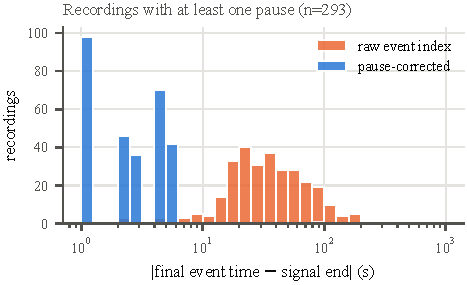
\includegraphics[width=0.7\textwidth]{figures/alignment.pdf}
\caption{Offset between the final \textit{Paused} event and the end of the signal for recordings with
pauses, before (orange) and after (blue) the correction.}
\label{fig:align}
\end{figure}

\textbf{State timeline and clean mask.} From the corrected events we label every second as eyes-closed,
eyes-open, photic, hyperventilation or unknown. A clean mask removes 1\,s before and 3\,s after every state
change, 3\,s around pause joins, 2\,s before to 3\,s after point artifacts (movement, coughing, swallowing,
talking) and 30\,s after drowsiness or sleep annotations. Hyperventilation, which slows the EEG of healthy
subjects, is excluded from both segments and biomarkers.

\subsection{Age-Normative Clinical Biomarkers}
For each recording we compute 48 biomarkers from Welch spectra of 4\,s windows (2\,s step):
\begin{itemize}[leftmargin=*,itemsep=0pt,topsep=2pt]
\item \textit{Eyes-closed (39):} log relative $\delta$, $\theta$, $\alpha$ and $\beta$ power in five regions;
      theta/alpha, delta/alpha and slow/fast ratios; fronto-posterior alpha ratio; alpha and beta hemispheric
      asymmetry; posterior alpha centre of gravity and peak frequency; spectral entropy; median frequency;
      total power; Hjorth mobility and complexity; inter-hemispheric and fronto-posterior coherence.
\item \textit{Eyes-open (5):} global relative band powers and posterior alpha centre of gravity.
\item \textit{Reactivity and driving (2):} posterior alpha reactivity, $\log(P_\alpha^{EC}/P_\alpha^{EO})$, and
      occipital photic-driving signal-to-noise ratio at the flash frequency.
\item \textit{Availability (2):} indicators for the presence of eyes-open and photic data.
\end{itemize}
Because EEG slows with healthy ageing, a raw biomarker mixes age with impairment. For every biomarker $x_j$ we
fit a linear age model on the \emph{training Normal recordings only} and replace $x_j$ with its robust
deviation
\begin{equation}
z_j = \frac{x_j - f_j(\text{age})}{1.4826\,\mathrm{MAD}_j},
\end{equation}
where $\mathrm{MAD}_j$ is the median absolute deviation of the normal residuals; values are clipped to
$\pm6$. In cross-validation the normative model is refitted within each fold.

\subsection{Evaluation Protocol}
All metrics are per recording and all splits are patient-disjoint. We report two complementary protocols.
(i) \textbf{Official split}, the benchmark protocol of \citet{kim2023caueeg}: models are trained on the 950
training recordings and scored on the 118 test recordings and the 90-recording no-overlap subset.
(ii) \textbf{Repeated five-fold cross-validation} over the pooled 1,069 training and validation recordings,
with the normative model and age scaling refitted in each fold, giving one out-of-fold prediction per
recording; the main models are run with several fold assignments. Metrics are accuracy, balanced accuracy,
macro F1, macro one-vs-rest area under the ROC curve (AUC), per-class recall and pairwise AUCs, with 95\%
bootstrap confidence intervals (1,000 resamples); model differences use a paired bootstrap on the same
recordings.

\section{Baseline Models and Results}

\subsection{Baseline Models}
All baselines use exactly the same folds, per-fold normative refitting and per-recording scoring as the
proposed model.

\textbf{Tabular models.} Age alone; the 48 biomarkers, raw or normative; and normative biomarkers plus age.
Each uses $L_2$-regularised, class-balanced logistic regression (LR), with the regularisation strength tuned by
an inner five-fold cross-validation. The last set is also modelled with histogram gradient boosting (HGB).

\textbf{Deep models on raw EEG.} EEGNet-8,2 \citep{lawhern2018eegnet} and a CEEDNet-style 1D-ResNet (four stages
of two residual blocks on the raw 19 channels, age concatenated before the classifier, 2.3M parameters)
\citep{kim2023caueeg}, both trained on random 10\,s crops. Both share the proposed model's data pipeline,
loss, schedule, augmentation and weight averaging, and average segment logits per recording, so only the
architecture differs. The 1D-ResNet follows CEEDNet's design but is not the authors' code or training recipe.

\subsection{Baseline Results}
Table~\ref{tab:baselines} lists the baselines. The tabular models are strong: age alone already reaches
51.1\% (AUC 0.709), and logistic regression on normative biomarkers plus age reaches $59.3\pm0.7\%$ (AUC
$0.778\pm0.004$). The deep models that see only raw EEG are weaker: EEGNet reaches 52.9\% (AUC 0.707) and the
1D-ResNet 57.7\% (AUC 0.752). On the official test split the 1D-ResNet scores 61.0\%, below the published
70.2\% for CEEDNet, which used larger models, longer training and test-time augmentation.

\begin{table}[H]
\centering
\caption{Baseline results (per recording). Cross-validation: five-fold out-of-fold, $n=1069$ (mean $\pm$
s.d.\ over five fold assignments where marked $^\ast$). Test: official test split, $n=118$, mean of the five
fold models}
\label{tab:baselines}
\small
\begin{tabular}{lcccccc}
\toprule
& \multicolumn{3}{c}{Cross-validation} & \multicolumn{3}{c}{Official test}\\
\cmidrule(lr){2-4}\cmidrule(lr){5-7}
Model & Acc & BAcc & AUC & Acc & BAcc & AUC\\
\midrule
Age (LR)$^\ast$ & $51.1\pm0.2$ & $51.6\pm0.2$ & $.709\pm.002$ & 55.1 & 54.6 & .739\\
Biomarkers, raw (LR) & 56.0 & 56.0 & .761 & 63.6 & 63.5 & .815\\
Biomarkers, normative (LR) & 58.1 & 58.1 & .761 & 62.7 & 63.2 & .809\\
Normative biomarkers + age (LR)$^\ast$ & $59.3\pm0.7$ & $59.3\pm0.7$ & $.778\pm.004$ & 66.1 & 65.9 & .839\\
Normative biomarkers + age (HGB) & 59.2 & 58.9 & .779 & 61.0 & 60.2 & .813\\
EEGNet & 52.9 & 51.5 & .707 & 60.2 & 58.0 & .773\\
1D-ResNet (CEEDNet-style) & 57.7 & 57.1 & .752 & 61.0 & 60.0 & .810\\
\bottomrule
\end{tabular}\\[2pt]
\parbox{\textwidth}{\scriptsize Acc: accuracy (\%); BAcc: balanced accuracy (\%); AUC: macro one-vs-rest area under
the ROC curve; LR: logistic regression; HGB: histogram gradient boosting.}
\end{table}

\section{Proposed Model: SANF-Net}

SANF-Net (\textbf{S}tate-\textbf{A}ware, age-\textbf{N}ormative \textbf{F}usion \textbf{Net}work) has three input
branches combined by modality-gated fusion (Figure~\ref{fig:arch}). It has 143k parameters.

\begin{figure}[H]
\centering
\resizebox{0.85\textwidth}{!}{% SANF-Net architecture (TikZ). Included from main.tex with % SANF-Net architecture (TikZ). Included from main.tex with \input{figures/architecture}.
\begin{tikzpicture}[
  font=\scriptsize, >=stealth,
  blk/.style={draw=black!60, rounded corners=1.5pt, align=center, inner sep=2pt,
              minimum height=8mm, text width=#1},
  blk/.default=19mm,
  arr/.style={->, draw=black!65, line width=0.5pt}]
\def\ya{0} \def\yb{-1.15} \def\yc{-2.1}

% inputs
\node[blk, fill=blue!8]    (seg) at (0,\ya) {EEG segments\\$19{\times}1000$, state $s$};
\node[blk, fill=orange!10] (bm)  at (0,\yb) {48 normative\\biomarkers $z$};
\node[blk, fill=black!6]   (ag)  at (0,\yc) {age};

% branches
\node[blk=16mm, fill=blue!8]    (enc)  at (2.25,\ya) {multi-scale\\CNN + SE};
\node[blk=10mm, fill=blue!8]    (film) at (3.75,\ya) {FiLM\\($s$)};
\node[blk=12mm, fill=blue!8]    (pool) at (5.15,\ya) {gated\\attention};
\node[blk=16mm, fill=orange!10] (bmlp) at (2.25,\yb) {MLP $\to$ 64};
\node[blk=16mm, fill=black!6]   (amlp) at (2.25,\yc) {MLP $\to$ 16};

% fusion (spans the biomarker and age rows)
\node[draw=black!60, rounded corners=1.5pt, fill=teal!10, align=center, text width=14mm,
      minimum height=19mm] (fuse) at (5.15,{(\yb+\yc)/2}) {modality-\\gated\\fusion\\[1pt]$\sum_m g_m h_m$};

% heads and output
\node[blk=15mm, fill=teal!10] (soft) at (7.05,\yb) {softmax\\(focal CE)};
\node[blk=15mm, fill=teal!10] (ord)  at (7.05,\yc) {ordinal\\$\sigma(s_{\mathrm{sev}}{-}t_k)$};
\node[draw=black!60, rounded corners=1.5pt, align=center, text width=15mm, minimum height=8mm]
      (out) at (9.0,{(\yb+\yc)/2}) {average\\N/MCI/D};

\draw[arr] (seg) -- (enc);
\draw[arr] (enc) -- (film);
\draw[arr] (film) -- (pool);
\draw[arr] (pool) -- (fuse);
\draw[arr] (bm) -- (bmlp);
\draw[arr] (ag) -- (amlp);
\draw[arr] (bmlp) -- (bmlp -| fuse.west);
\draw[arr] (amlp) -- (amlp -| fuse.west);
\draw[arr] (fuse.east |- soft) -- (soft);
\draw[arr] (fuse.east |- ord) -- (ord);
\draw[arr] (soft.east) -- (out);
\draw[arr] (ord.east) -- (out);
\node[font=\tiny, color=black!60, above=0.3mm of enc] {shared over 12--24 segments};
\end{tikzpicture}
.
\begin{tikzpicture}[
  font=\scriptsize, >=stealth,
  blk/.style={draw=black!60, rounded corners=1.5pt, align=center, inner sep=2pt,
              minimum height=8mm, text width=#1},
  blk/.default=19mm,
  arr/.style={->, draw=black!65, line width=0.5pt}]
\def\ya{0} \def\yb{-1.15} \def\yc{-2.1}

% inputs
\node[blk, fill=blue!8]    (seg) at (0,\ya) {EEG segments\\$19{\times}1000$, state $s$};
\node[blk, fill=orange!10] (bm)  at (0,\yb) {48 normative\\biomarkers $z$};
\node[blk, fill=black!6]   (ag)  at (0,\yc) {age};

% branches
\node[blk=16mm, fill=blue!8]    (enc)  at (2.25,\ya) {multi-scale\\CNN + SE};
\node[blk=10mm, fill=blue!8]    (film) at (3.75,\ya) {FiLM\\($s$)};
\node[blk=12mm, fill=blue!8]    (pool) at (5.15,\ya) {gated\\attention};
\node[blk=16mm, fill=orange!10] (bmlp) at (2.25,\yb) {MLP $\to$ 64};
\node[blk=16mm, fill=black!6]   (amlp) at (2.25,\yc) {MLP $\to$ 16};

% fusion (spans the biomarker and age rows)
\node[draw=black!60, rounded corners=1.5pt, fill=teal!10, align=center, text width=14mm,
      minimum height=19mm] (fuse) at (5.15,{(\yb+\yc)/2}) {modality-\\gated\\fusion\\[1pt]$\sum_m g_m h_m$};

% heads and output
\node[blk=15mm, fill=teal!10] (soft) at (7.05,\yb) {softmax\\(focal CE)};
\node[blk=15mm, fill=teal!10] (ord)  at (7.05,\yc) {ordinal\\$\sigma(s_{\mathrm{sev}}{-}t_k)$};
\node[draw=black!60, rounded corners=1.5pt, align=center, text width=15mm, minimum height=8mm]
      (out) at (9.0,{(\yb+\yc)/2}) {average\\N/MCI/D};

\draw[arr] (seg) -- (enc);
\draw[arr] (enc) -- (film);
\draw[arr] (film) -- (pool);
\draw[arr] (pool) -- (fuse);
\draw[arr] (bm) -- (bmlp);
\draw[arr] (ag) -- (amlp);
\draw[arr] (bmlp) -- (bmlp -| fuse.west);
\draw[arr] (amlp) -- (amlp -| fuse.west);
\draw[arr] (fuse.east |- soft) -- (soft);
\draw[arr] (fuse.east |- ord) -- (ord);
\draw[arr] (soft.east) -- (out);
\draw[arr] (ord.east) -- (out);
\node[font=\tiny, color=black!60, above=0.3mm of enc] {shared over 12--24 segments};
\end{tikzpicture}
}
\caption{SANF-Net. State-tagged EEG segments, age-normative biomarkers and age are encoded separately and
combined by modality-gated fusion feeding a softmax and an ordinal head.}
\label{fig:arch}
\end{figure}

\subsection{Architecture}

\textbf{EEG branch.} A recording is a bag of 10\,s segments ($19 \times 1000$ samples) drawn from clean seconds
by state: 60\% eyes-closed, 25\% eyes-open and 15\% photic (12 segments per recording in training, 24 at
evaluation). A shared encoder applies three parallel temporal convolutions (0.11, 0.25 and 0.51\,s kernels,
matching beta, alpha and delta--theta time scales), a depthwise spatial convolution over the 19 channels, a
separable convolution with squeeze-and-excitation (SE), a temporal convolution with a second SE block, and
mean and standard-deviation pooling to a 128-dimensional embedding $h$. Each embedding is modulated by its
state $s$ with feature-wise linear modulation (FiLM) \citep{perez2018film}, $h' = h\odot(1+\gamma_s)+\beta_s$,
and gated attention pooling \citep{ilse2018attention} combines the segments of a recording.

\textbf{Biomarker and age branches.} The 48 normative $z$-scores pass through a two-layer perceptron
(64-dimensional output) and standardised age through a small perceptron (16-dimensional). Age is an explicit
input so that its contribution can be measured and ablated.

\textbf{Modality-gated fusion.} Each branch is projected to 128 dimensions; a linear layer over the
concatenated projections yields softmax gates $g$ over the three modalities, and the fused vector is
$\sum_m g_m h_m$. The gates show how much each prediction relied on EEG, biomarkers or age. During training
each modality is dropped with probability 0.15 (never all at once), so that no single input, particularly age,
carries the model.

\textbf{Two output heads.} Normal $<$ MCI $<$ Dementia is an ordered scale. Besides a softmax head, an ordinal
cumulative-link head \citep{mccullagh1980regression} predicts a severity score $s_{\mathrm{sev}}$ and two
ordered thresholds $t_1<t_2$, with $P(y>k)=\sigma(s_{\mathrm{sev}}-t_k)$. The class probabilities of the two
heads are averaged.

\subsection{Training}
The loss is a class-weighted focal cross-entropy \citep{lin2017focal} ($\gamma=1.5$; weights 1.0 / 1.4 / 1.2 for
Normal / MCI / Dementia; label smoothing 0.05) plus 0.5 times the cumulative binary cross-entropy of the
ordinal head. We train for 35 epochs with AdamW (learning rate $10^{-3}$, weight decay 0.05, three-epoch
warm-up and cosine decay), 16 recordings per batch, mixed precision, gradient clipping at 2.0 and an
exponential moving average (EMA) of the weights (decay 0.995). Augmentation comprises amplitude scaling
(0.9--1.1), Gaussian noise, channel dropout (0.1), biomarker noise and \emph{same-class bag mixing}: with
probability 0.3, 25--50\% of a recording's segments are replaced by segments of another training recording
with the same label. We evaluate the final EMA weights rather than selecting a checkpoint on the small
validation set, whose 119 recordings make checkpoint selection noisy. One model trains in about 6 minutes on
a laptop RTX~4050 GPU. Table~\ref{tab:hparams} summarises the configuration.

\begin{table}[H]
\centering
\caption{SANF-Net configuration}
\label{tab:hparams}
\small
\begin{tabular}{ll@{\hspace{2em}}ll}
\toprule
Setting & Value & Setting & Value\\
\midrule
Sampling rate & 100\,Hz & Parameters & 143k\\
Band-pass & 0.5--45\,Hz & Epochs & 35\\
Segment length & 10\,s ($19\times1000$) & Batch & 16 recordings\\
Segments (train / eval) & 12 / 24 & Optimiser & AdamW, lr $10^{-3}$, wd 0.05\\
State mix (EC / EO / photic) & 60 / 25 / 15\% & Loss & focal ($\gamma$ 1.5) + 0.5 ordinal\\
Biomarkers & 48, age-normative & Class weights & 1.0 / 1.4 / 1.2\\
Temporal kernels & 0.11 / 0.25 / 0.51\,s & Dropout / modality dropout & 0.3 / 0.15\\
Embedding / fusion size & 128 / 128 & Weight averaging & EMA, decay 0.995\\
\bottomrule
\end{tabular}
\end{table}

\section{Ensemble and Results}

\subsection{Final Ensemble}
The final model is an ensemble of three SANF-Net instances trained on the official training split with
different random seeds and identical settings. For each recording the class probabilities of the three
models are averaged and the most probable class is predicted. The ensemble has 429k parameters in total.

\subsection{Official Test Results}
Table~\ref{tab:main} compares SANF-Net with the published CEEDNet results on the official test split. The
ensemble reaches \textbf{72.9\% accuracy}, 72.3\% balanced accuracy, a macro F1 of 0.709 and a \textbf{macro AUC
of 0.870}. A single SANF-Net reaches $68.4\pm2.8\%$ (individual seeds 64.4\%, 70.3\% and 70.3\%). The ensemble
is above CEEDNet's best single model (70.2\%) and within 1.8 points of its nine-model ensemble (74.7\%), with
about 590 times fewer parameters. On the no-overlap subset, which excludes every patient seen in training, the
ensemble reaches 72.2\% (AUC 0.863), close to its full-test score, which indicates no leakage through repeated
patients. CEEDNet's ensemble reports 76.7\% on this subset. With 118 test recordings, the 95\% confidence
interval of any single test accuracy is about $\pm8$ points.

\begin{table}[H]
\centering
\caption{Three-class results on the official CAUEEG split (per recording). Single SANF-Net: mean $\pm$ s.d.\
over three seeds}
\label{tab:main}
\small
\begin{tabular}{lrcccccc}
\toprule
& & \multicolumn{4}{c}{Test ($n=118$)} & \multicolumn{2}{c}{No-overlap ($n=90$)}\\
\cmidrule(lr){3-6}\cmidrule(lr){7-8}
Model & Params & Acc & BAcc & F1 & AUC & Acc & AUC\\
\midrule
CEEDNet, best single model$^\dagger$ & 11M+ & 70.2 & -- & -- & -- & -- & --\\
CEEDNet, 9-model ensemble$^\dagger$ & 253.8M & 74.7 & -- & -- & -- & 76.7 & --\\
\midrule
SANF-Net, single & 143k & $68.4\pm2.8$ & $67.3\pm3.6$ & $.666\pm.035$ & $.849\pm.014$ & $67.4\pm1.4$ & $.844\pm.011$\\
\textbf{SANF-Net, 3-model ensemble} & 429k & \textbf{72.9} & \textbf{72.3} & \textbf{.709} & \textbf{.870} & \textbf{72.2} & \textbf{.863}\\
\bottomrule
\end{tabular}\\[2pt]
\parbox{\textwidth}{\scriptsize $^\dagger$As published by \citet{kim2023caueeg}, with their own training recipe and
test-time augmentation. Params: parameters; F1: macro F1.}
\end{table}

\textbf{Per-class performance.} Table~\ref{tab:perclass} gives the ensemble's confusion matrix and per-class
metrics. The model recognises 95.7\% of healthy participants and labels none of them as demented, and detects
77.4\% of dementia patients. MCI is the hardest class: its recall is 43.9\%, with errors split between the
two neighbouring classes, but its precision is the highest of all classes (75.0\%), so an MCI prediction is
usually correct. Severe errors (Normal predicted as Dementia or the reverse) are rare.

\begin{table}[H]
\centering
\caption{Confusion matrix (row percentages, counts in brackets) and per-class metrics of the SANF-Net ensemble
on the official test split}
\label{tab:perclass}
\small
\begin{tabular}{lccc@{\hspace{2em}}ccc}
\toprule
True $\downarrow$ / Predicted $\rightarrow$ & Normal & MCI & Dementia & Precision & Recall & F1\\
\midrule
Normal ($n=46$) & \textbf{95.7} (44) & 4.3 (2) & 0.0 (0) & 72.1 & 95.7 & .822\\
MCI ($n=41$) & 34.1 (14) & \textbf{43.9} (18) & 22.0 (9) & 75.0 & 43.9 & .554\\
Dementia ($n=31$) & 9.7 (3) & 12.9 (4) & \textbf{77.4} (24) & 72.7 & 77.4 & .750\\
\bottomrule
\end{tabular}
\end{table}

\textbf{What the model uses.} The mean modality gates on the test set differ by true class. For Normal
recordings the EEG branch has the largest weight (EEG 0.39, biomarkers 0.29, age 0.32); for MCI the biomarker
and age branches dominate (0.37 and 0.38, EEG 0.25); for Dementia the three are balanced (0.34, 0.35, 0.31).

\subsection{Cross-Validated Results}
Because a 118-recording test set is small and the official test split turns out to be easier than the pooled
data (the same models score $59.9\pm1.0\%$ on validation but $68.4\pm2.8\%$ on test), we also evaluate under
repeated five-fold cross-validation. SANF-Net reaches $59.5\pm0.3\%$ accuracy and a macro AUC of
$0.778\pm0.006$ over four fold assignments (first assignment: 59.8\%, 95\% CI 56.7--62.8\%), which is very stable
across repeats. Under the identical protocol it is significantly better than EEGNet ($+6.8$ points, CI
3.4--10.1) and better than the 1D-ResNet in AUC ($+0.028$, CI 0.003--0.050), and it is statistically
indistinguishable from logistic regression on the same normative biomarkers plus age (paired difference
$-0.1\pm0.5$ points). Out-of-fold recall is 76.8\% for Normal, 62.9\% for Dementia and 38.8\% for MCI
(Figure~\ref{fig:cm}). For MCI versus Normal the AUC is 0.787, detecting 63\% of MCI at 80\% specificity.

\begin{figure}[H]
\centering
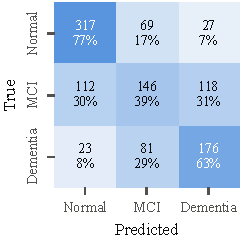
\includegraphics[width=0.45\textwidth]{figures/confusion.pdf}
\caption{SANF-Net out-of-fold confusion matrix under five-fold cross-validation ($n=1069$, counts and row
percentages).}
\label{fig:cm}
\end{figure}

\subsection{Ablation Study}
Table~\ref{tab:ablation} removes one component at a time under the same cross-validation protocol. Removing
both non-EEG branches clearly hurts: the EEG-only network loses 4.5 accuracy points (CI 1.4--8.0) and 0.049
macro AUC, and its MCI recall falls to 24.5\%. State-aware sampling gives a small but significant AUC gain
($+0.013$, CI 0.002--0.025), and normative scoring and the biomarker branch each add about 0.02 MCI-versus-Normal
AUC. Removing the ordinal head leaves accuracy and AUC unchanged but raises MCI recall from 38.8\% to 58.8\%,
at the cost of Normal and Dementia recall; this gives a screening-oriented operating point.

\begin{table}[H]
\centering
\caption{Ablations (five-fold cross-validation, out-of-fold, $n=1069$)}
\label{tab:ablation}
\small
\begin{tabular}{lcccc}
\toprule
Variant & Acc & AUC & AUC Normal vs MCI & MCI recall\\
\midrule
SANF-Net (full) & 59.8 & .780 & .787 & 38.8\\
\quad random crops, no state & 58.6 & .767 & .781 & 36.2\\
\quad no FiLM state conditioning & 58.9 & .777 & .784 & 41.8\\
\quad mean instead of attention pooling & 58.5 & .782 & .783 & 35.9\\
\quad plain standardisation (no normative) & 57.6 & .768 & .768 & 36.4\\
\quad no biomarkers & 57.3 & .772 & .767 & 34.8\\
\quad no age & 58.5 & .783 & .788 & 37.0\\
\quad EEG only & 55.3 & .731 & .719 & 24.5\\
\quad no ordinal head & 59.5 & .777 & .785 & 58.8\\
\bottomrule
\end{tabular}
\end{table}

\subsection{Protocol and Age Confounds}
Community-recruited normals differ from every other group in ways unrelated to cognition
(Table~\ref{tab:groups}, Figure~\ref{fig:protocol}): they are younger (61.7 versus 69.6--76.6 years), only 12\%
of their recordings include photic stimulation (versus 90--92\% of every other group), and their recordings
are shorter. A model can therefore recognise many community normals from the protocol alone.

\begin{figure}[H]
\centering
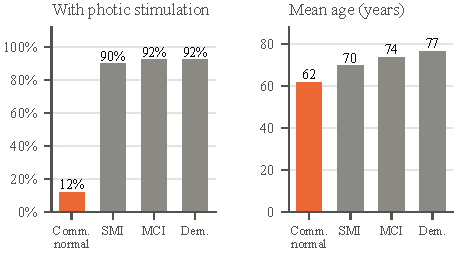
\includegraphics[width=0.7\textwidth]{figures/protocol.pdf}
\caption{Share of recordings with photic stimulation and mean age per subgroup. Community normals differ from
all clinical groups in both, independently of cognition.}
\label{fig:protocol}
\end{figure}

We therefore trained protocol-blind variants: (A) SANF-Net with photic segments and the three protocol
features removed, and (B) SANF-Net on eyes-closed segments only (Table~\ref{tab:confound}). Removing protocol
information costs SANF-Net 2.7 accuracy points and the linear model 2.5 points, almost entirely on the
community-versus-MCI comparison, whereas SMI-versus-MCI stays at 0.65--0.66 for every model. SANF-Net relies
less on the shortcut than the linear model, as its much higher SMI recall shows (57.9\% versus 35.7\%). After
1:1 age matching, SMI versus MCI falls to 0.54--0.57 for every model, and the 24 community normals recorded
with photic stimulation are not distinguished from age-matched MCI by any model (AUC 0.50--0.59).

\begin{table}[H]
\centering
\caption{Protocol confound (five-fold cross-validation, out-of-fold). Comm.: community-recruited normals
($n=229$); SMI: subjective memory impairment ($n=171$)}
\label{tab:confound}
\small
\begin{tabular}{lccccc}
\toprule
& & & \multicolumn{2}{c}{AUC vs MCI} & \\
\cmidrule(lr){4-5}
Model & Acc & AUC & Comm. & SMI & SMI recall\\
\midrule
Age (LR) & 51.1 & .709 & .858 & .618 & 42.7\\
Normative biomarkers + age (LR) & 59.3 & .778 & .951 & .655 & 35.7\\
\quad without protocol features & 56.8 & .747 & .863 & .660 & 50.6\\
SANF-Net & 59.8 & .780 & .891 & .653 & 57.9\\
\quad (A) no photic information & 57.1 & .764 & .852 & .649 & 63.7\\
\quad (B) eyes-closed only & 58.5 & .756 & .842 & .650 & 63.7\\
\bottomrule
\end{tabular}
\end{table}

\subsection{External Validation}
Table~\ref{tab:external} reports MCI-versus-normal performance on the external cohorts without retraining, using
the five cross-validation fold models (predictions averaged); MCI is scored with $1-P(\text{Normal})$. Since age
is uninformative there, these results reflect EEG and biomarkers only. We also apply a label-free \emph{site
calibration}: channel amplitudes are rescaled to the cohort's median and the normative $z$-scores are
re-centred on the cohort's own normals in a leave-one-out manner. On the pooled Isfahan cohorts the AUC is
0.67, rising to \textbf{0.70} with site calibration (0.76 on Isfahan 2016); on GENEEG, whose montage and
protocol differ more, it is 0.58. Across the external cohorts 81--91\% of healthy participants are correctly
classified as Normal. With 61--63 subjects per cohort all intervals are wide.

\begin{table}[H]
\centering
\caption{External MCI versus normal without retraining. AUC with 95\% bootstrap confidence interval}
\label{tab:external}
\small
\begin{tabular}{lccc}
\toprule
Cohort & $n$ (MCI) & No calibration & Site calibration\\
\midrule
Isfahan 2016 & 27 (11) & .73 (.51--.91) & .76 (.57--.92)\\
Isfahan 2019 & 34 (18) & .64 (.45--.84) & .63 (.44--.81)\\
Isfahan pooled & 61 (29) & .67 (.53--.80) & .70 (.56--.83)\\
GENEEG & 63 (28) & .58 (.44--.72) & .58 (.42--.74)\\
\bottomrule
\end{tabular}
\end{table}

\begin{figure}[H]
\centering
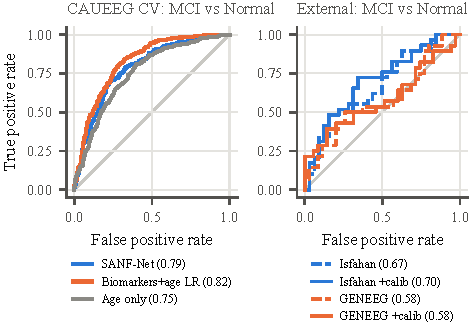
\includegraphics[width=0.85\textwidth]{figures/roc.pdf}
\caption{MCI versus normal ROC curves. Left: CAUEEG out-of-fold predictions. Right: external cohorts without
retraining, with and without site calibration.}
\label{fig:roc}
\end{figure}

% \section{Clinical Dashboard}

% =========================== PLACEHOLDER =====================================
% Replace this section once the dashboard is built. Suggested content:
%   - purpose and intended user (clinician / EEG technician)
%   - workflow: upload EDF + event file -> preprocessing -> SANF-Net ensemble -> report
%   - what is shown: predicted class and probabilities, modality gates (EEG /
%     biomarkers / age), key biomarker z-scores against age-matched normals,
%     recording-state timeline and clean-signal coverage
%   - technology stack and inference time
%   - one or two screenshots (Figure X)
% ==============================================================================

\todo{Describe the clinician-facing dashboard: purpose, workflow from EEG upload to prediction, displayed
outputs (class probabilities, modality gates, age-normative biomarker deviations, state timeline), technology
stack and inference time.}

\begin{figure}[H]
\centering
\fbox{\parbox[c][5cm][c]{0.8\textwidth}{\centering\textcolor{red}{[Dashboard screenshot placeholder]}}}
\caption{\todo{Dashboard screenshot and caption.}}
\label{fig:dashboard}
\end{figure}
   % add back once the dashboard is built
\section{Discussions}

\textbf{A compact model at benchmark level.} The SANF-Net ensemble reaches 72.9\% accuracy and an AUC of 0.87 on
the official test split with 429k parameters, above CEEDNet's best single model and close to its nine-model
ensemble, which is about 590 times larger. A model of this size trains in minutes on a laptop GPU and is
suitable for portable or primary-care hardware, which is where an EEG-based screen is most useful. Its
clinical error profile is favourable for screening: almost all healthy participants are recognised, no healthy
participant is labelled as demented, and when MCI is predicted it is usually correct.

\textbf{The recording state matters.} Correcting the event clock was a prerequisite for state-aware sampling,
for the alpha-reactivity and photic-driving biomarkers, and for detecting the protocol confound. State-aware
sampling gives a significant AUC gain over random crops, and the gates make each prediction's reliance on EEG,
biomarkers and age visible.

\textbf{Architecture versus features.} Under cross-validation SANF-Net matches, but does not beat, logistic
regression on the same normative biomarkers, and it beats the EEG-only deep baselines mainly because it also
sees the biomarkers and age: its own EEG-only ablation lies between EEGNet and the 1D-ResNet. Gains on this
benchmark should therefore always be compared against a strong tabular model of established markers under the
same protocol. SANF-Net's advantage over the linear model is that it relies far less on the protocol shortcut.

\textbf{Much of the MCI signal is age and protocol.} The MCI-versus-Normal AUCs on CAUEEG mix age, recording
protocol and EEG physiology. After age matching, distinguishing a patient with memory complaints who does or
does not have MCI reaches only 0.54--0.57, consistent with the overlapping feature distributions reported by
\citet{geneeg2025}. Results on this dataset should be reported per Normal subgroup and with age-matched
comparisons.

\textbf{Single splits mislead.} The official test split is about 8 points easier than the pooled data, and a
118-recording test set carries an interval of about $\pm8$ points. Cross-validated results with repeated fold
assignments should accompany any official-test number.

\textbf{Transfer.} Without retraining or age information, the model keeps useful MCI discrimination on Isfahan
(AUC 0.67--0.76) and recognises most healthy participants at new sites, but transfers little to GENEEG, whose
montage and protocol differ more. Re-centring normative references on a site's own normals is cheap and
label-free.

\textbf{Limitations.} Training data come from a single hospital. The model design was developed on the
official split and the official test set was consulted during development, which is one reason
cross-validated results are reported alongside it. Subgroup labels rely on the dataset's symptom codes, and the
community-with-photic subgroup is small. The external cohorts are small, lack ages and state annotations, and
were not recorded with the CAUEEG protocol. Diagnoses are clinical, without biomarker confirmation.

\section{Conclusions}

CAUEEG event annotations need a pause correction before they can be used. Once corrected, they enable
state-aware, age-normative modelling of MCI and dementia. SANF-Net, a 143k-parameter fusion network built on
these ideas, reaches 72.9\% accuracy and an AUC of 0.87 on the official test split as a three-model ensemble,
comparable to published models hundreds of times larger, with interpretable modality gates. Under repeated
cross-validation it reaches 59.5\%, outperforms deep EEG-only baselines, matches a strong linear model while
relying less on the protocol shortcut, and transfers to an independent cohort with an AUC of 0.70. The analysis
also shows that community-recruited normals in CAUEEG are distinguishable by recording protocol and age alone,
so confound-controlled, cross-validated evaluation should be standard for EEG-based cognitive screening.
Future work includes improving MCI sensitivity, multi-site training, adding cognitive test scores, and
deploying the model through a clinician-facing dashboard.

% Back matter in the order required by the IJCRSEE template.

\section{Acknowledgements}
We thank our guide, Dr.\ Sujata Kulkarni, for her guidance throughout the project, and the creators of the
CAUEEG, Isfahan MCI and GENEEG datasets for making their data available.

\section{Funding}
This research did not receive any specific grant from funding agencies in the public, commercial, or
not-for-profit sectors.

\section{Conflict of Interests}
The authors declare no conflict of interest.

\section{Data Availability Statement}
The data that support the findings of this study are available from their original providers. These data were
derived from the following resources: the CAUEEG dataset \citep{kim2023caueeg}, the Isfahan MCI datasets
\citep{kashefpoor2016automatic,kashefpoor2019supervised} and the GENEEG dataset \citep{geneeg2025}, under the
access conditions of each provider. The code, event-alignment correction, trained-model results and evaluation protocol are available at
\url{https://github.com/nityaashetty/SidMajor}.

\section{Institutional Review Board Statement}
Not applicable. This study is a secondary analysis of publicly available, de-identified datasets; no new data
were collected from human participants.

\section{Author Contributions}
All authors contributed equally to conceptualization, methodology, software, formal analysis, and writing
(original draft preparation, review and editing). All authors have read and agreed to the final version of
the manuscript.


% ============================ references ========================================
\renewcommand{\bibsection}{\section{References}}
\bibliographystyle{apalike}
\bibliography{references}

\end{document}
